\documentclass[11pt]{article}
\usepackage[margin=0.7in]{geometry}
\usepackage{multirow}
\usepackage {graphicx}
\usepackage[utf8x]{inputenc} % указать кодировку русского текста
\usepackage[russian]{babel} % указать, что язык текста - русский
\usepackage{fancyhdr}
\pagestyle{fancy}

\begin{document}

\begin{titlepage}

\begin{center}
%\vspace*{1cm}
\large\textbf{Московский Физико-Технический Институт}\\
\large\textbf{(государственный университет)}
\vfill
\line(1,0){430}\\[1mm]
\huge\textbf{Исследование взаимной диффузии газов}\\
\line(1,0){430}\\[1mm]
\vfill
\large Сибгатуллин Булат, ФРКТ\\
\end{center}

\end{titlepage}
\fancyhead[L] {Работа 2.3.1}
\noindent \textbf{Цель работы:} \\
\indent 1) измерение объемов форвакуумной и высоковакуумной частей установки; 2) определение скорости откачки системы в стационарном режиме, а также по ухудшению и по улучшению вакуума.\\
\noindent \textbf{В работе используются:} \\
\indent вакуумная установка №3 с манометрами: масляным,  термопарным  и ионизационным.
\section*{Описание работы}\
\indent По степени разрежения вакуумные установки принято делить на три класса: 1) низковакуумные — до $10^{−2}$-$10^{−3}$ торр; 2) высоковакуумные — $10−4$–$10−7$ торр; 3) установки сверхвысокого вакуума — $10^{−8}$–$10^{−11}$  торр. В данной работе изучаются   традиционные методы откачки механическим форвакуумным насосом до давления $10^{−2}$ торр и диффузионным масляным насосом до давления $10^{−5}$ торр, а также методы измерения вакуума в этом диапазоне.\\
\ \\
\textbf{Экспериментальная установка:}\\
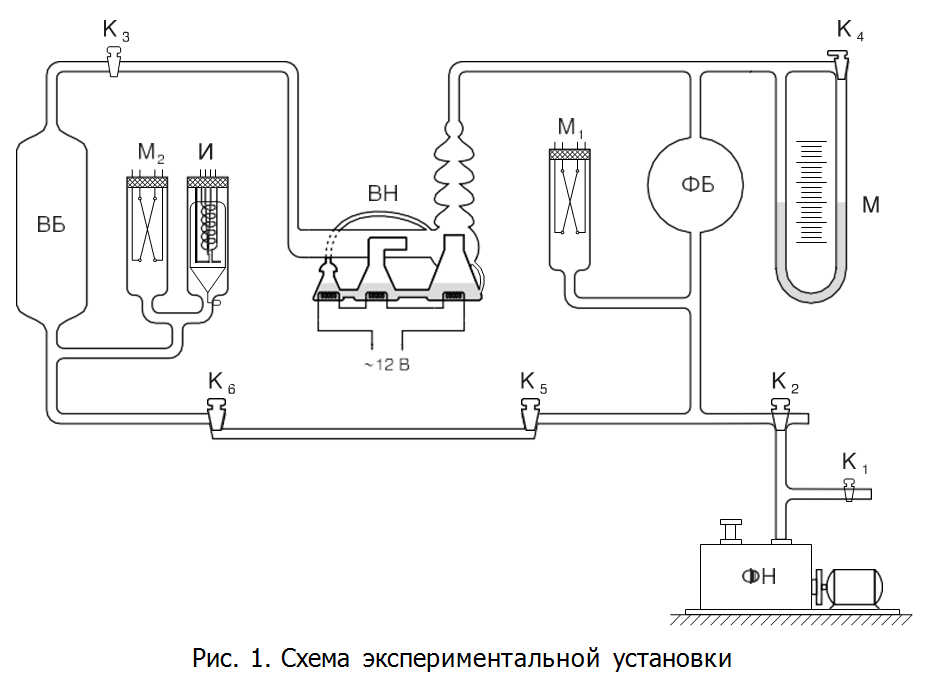
\includegraphics[scale=0.8]{pic1.png}
\newpage
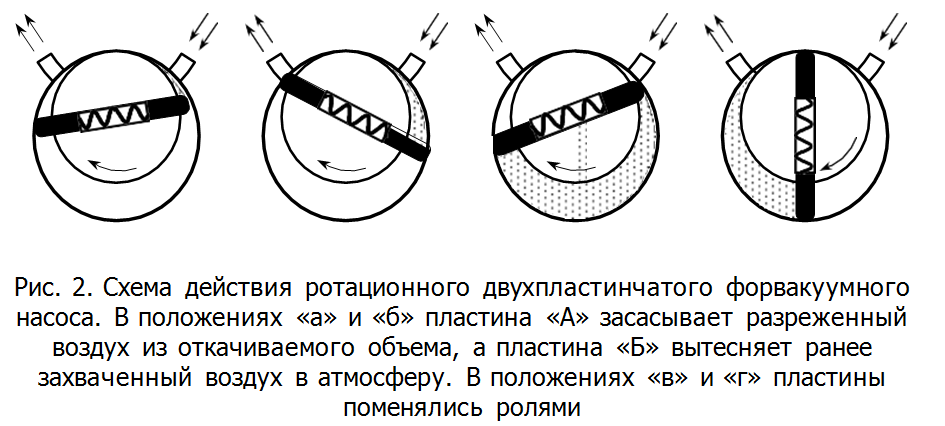
\includegraphics[scale=0.5]{pic2.png}
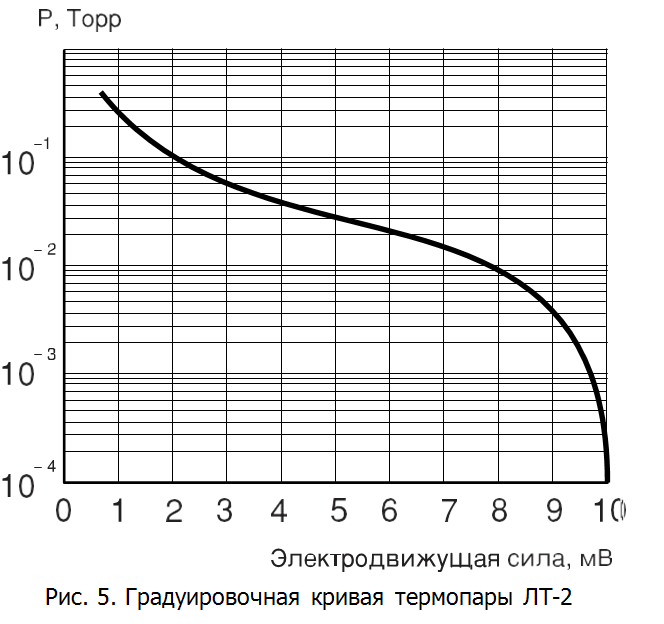
\includegraphics[scale=0.5]{pic5.png}\\
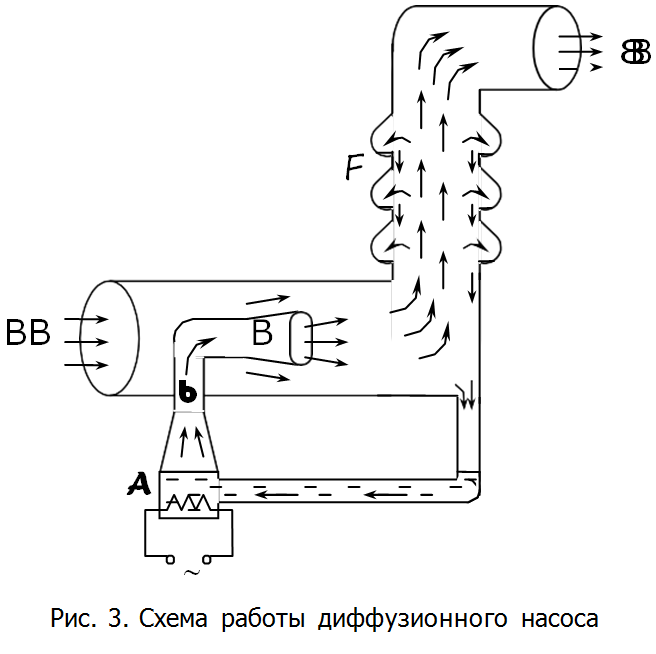
\includegraphics[scale=0.5]{pic3.png}
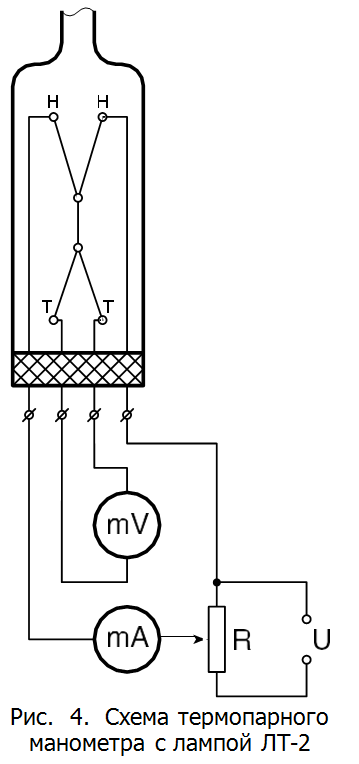
\includegraphics[scale=0.7]{pic4.png}
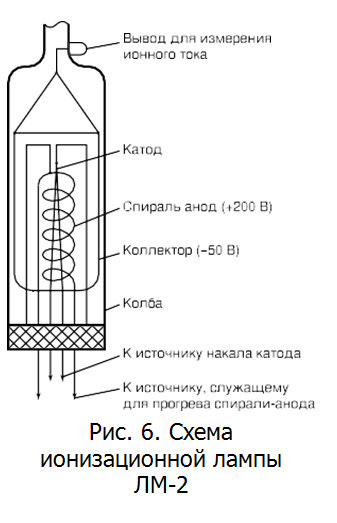
\includegraphics[scale=0.7]{pic6.png}
\newpage
\textbf{Процесс откачки.} Производительность насоса определяется скоростью откачки W (л/с): W — это объем газа, удаляемого из сосуда при данном давлении за единицу времени. Скорость откачки форвакуумного насоса равна емкости воздухозаборной камеры, умноженной на число оборотов в секунду.
Рассмотрим обычную схему откачки. Разделим вакуумную систему на две части: «откачиваемый объем» (в состав которого включим используемые для работы части установки) и «насос», к которому, кроме самого насоса, отнесем трубопроводы и краны, через которые
производится откачка нашего объема. Обозначим через $Q_d$ количество газа, десорбирующегося с поверхности откачиваемого объема в единицу времени, через $Q_i$ — количество газа, проникающего в единицу времени в этот объем извне — через течи. Будем считать, что насос обладает скоростью откачки W и в то же время сам является источником газа; пусть $Q_n$ — поток газа, поступающего из насоса назад в откачиваемую систему. Будем измерять количество газа $Q_d$, $Q_i$ и $Q_n$ в единицах PV (легко видеть, что это произведение с точностью до множителя RT/$\mu$ равно массе газа). Основное уравнение, описывающее процесс откачки, имеет вид
$$-VdP=(PW-Q_d-Q_n-Q_i)dt$$
Левая часть этого уравнения равна убыли газа в откачиваемом объеме V , а правая определяет количество газа, уносимого насосом, и количество прибывающего вследствие перечисленных выше причин
за время $dt$. При достижении предельного вакуума (давление $P_{pr}$)
$$\frac{dP}{dt}=0$$
$$W=\frac{\sum Q_i}{P_{pr}}$$
Обычно $Q_i$ постоянно, a $Q_n$ и $Q_d$ слабо зависят от времени, поэтому в наших условиях все эти члены можно считать постоянными. Считая также постоянной скорость откачки W , уравнение (1) можно проинтегрировать и, используя (2), получить
$$P=P_o exp(-\frac{W}{V}t) + P_{pr}$$
\textbf{Течение газа через трубу.}Характер течения газа существенно зависит от соотношения между размерами системы и длиной свободного пробега молекул. При атмосферном давлении и даже при понижении давления до форвакуумного длина свободного пробега меньше диаметра трубок и течение откачиваемого газа определяется его вязкостью, т. е. взаимодействием его молекул. При переходе к высокому вакууму картина меняется. Столкновения молекул между собой начинают играть меньшую роль, чем соударения со стенками. Течение газа в трубе напоминает в этих условиях диффузию газа из области больших концентраций в области, где концентрация ниже, причем роль длины свободного пробега играет ширина трубы.
Для количества газa, протекающего через трубу в условиях высокого вакуума или, как говорят, в кнудсеновском режиме, справедлива формула
$$\frac{d(PV)}{dt}=\frac{4}{3}r^3 \sqrt{\frac{2\pi RT}{\mu}} \frac{P_2-P_1}{L}$$
Применим эту формулу к случаю, когда труба соединяет установку с насосом.
Пренебрежем давлением P1 у конца, обращенного к насосу. Будем измерять количество газа, покидающего установку при давлении P =
= P2. Пропускная способность трубы
$$C_{tr}=(\frac{dV}{dt})_{tr}=\frac{4}{3}\frac{r^3}{L}\sqrt{\frac{2\pi RT}{\mu}}$$
Мы видим, что пропускная способность зависит от радиуса трубы в третьей степени и обратно пропорциональна ее длине. В вакуумных установках следует поэтому применять широкие короткие  трубы.
$$\frac{1}{W}=\frac{1}{W_n}+\frac{1}{C_1}+\frac{1}{C_2}+...$$
\newpage
\ \\
При расчете вакуумных систем нужно принимать во внимание также пропускную способность отверстий, например, в кранах. Для них имеется формула $$\eta=\frac{1}{4}Sn<v>$$
где $\eta$ — число молекул, вылетающих из отверстия в вакуум в единицу времени, S — площадь отверстия, n — концентрация молекул перед отверстием, <v> — средняя скорость молекул газа. С другой стороны, $\eta = dN/dt$, $N = PV/kT$ , $n = P/kT$ , и аналогично формуле для количества газа, покидающего установку при давлении P , получается пропускная способность отверстия
$$C_{otv}=(\frac{dV}{dt})_{otv}=S\frac{<v>}{4}$$
\ \\
Для диффузионного насоса можно считать, что каждая молекула воздуха, попавшая в кольцевой зазор между соплом и стенками насоса, увлекается струей пара и не возвращается обратно в откачиваемый объем. Скорость откачки такого насоса можно считать равной пропускной способности отверстия с площадью, равной площади кольцевого зазора, т. е. насос качает как кольцевой зазор, с одной стороны которого расположен откачиваемый объем, а с другой — пустота.


\end{document}